\documentclass[10pt]{article}
\usepackage{tikz}
\usepackage[margin=0cm]{geometry}
\pagestyle{empty}

\begin{document}

\vspace*{\fill}
\begin{center}
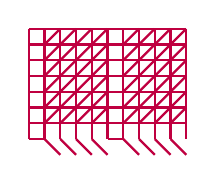
\begin{tikzpicture}[x=0.2cm, y=-0.2cm, thick, purple]
% North to South lines
    \draw (0,0) -- (0,7);
    \draw (1,0) -- (1,7);
    \draw (2,0) -- (2,7);
    \draw (3,0) -- (3,7);
    \draw (4,0) -- (4,7);
    \draw (5,0) -- (5,7);
    \draw (6,0) -- (6,7);
    \draw (7,0) -- (7,7);
    \draw (8,0) -- (8,7);
    \draw (9,0) -- (9,7);
    \draw (10,0) -- (10,7);
% North-West to South-East lines
    \draw (1,7) -- (2,8);
    \draw (2,7) -- (3,8);
    \draw (3,7) -- (4,8);
    \draw (4,7) -- (5,8);
    \draw (6,7) -- (7,8);
    \draw (7,7) -- (8,8);
    \draw (8,7) -- (9,8);
    \draw (9,7) -- (10,8);
% West to East lines
    \draw (0,0) -- (10,0);
    \draw (0,1) -- (10,1);
    \draw (0,2) -- (10,2);
    \draw (0,3) -- (10,3);
    \draw (0,4) -- (10,4);
    \draw (0,5) -- (10,5);
    \draw (0,6) -- (10,6);
    \draw (0,7) -- (1,7);
    \draw (5,7) -- (6,7);
% South-West to North-East lines
    \draw (1,1) -- (2,0);
    \draw (6,1) -- (7,0);
    \draw (1,2) -- (3,0);
    \draw (6,2) -- (8,0);
    \draw (1,3) -- (4,0);
    \draw (6,3) -- (9,0);
    \draw (1,4) -- (5,0);
    \draw (6,4) -- (10,0);
    \draw (1,5) -- (5,1);
    \draw (6,5) -- (10,1);
    \draw (1,6) -- (5,2);
    \draw (2,6) -- (5,3);
    \draw (3,6) -- (5,4);
    \draw (4,6) -- (5,5);
    \draw (6,6) -- (10,2);
    \draw (7,6) -- (10,3);
    \draw (8,6) -- (10,4);
    \draw (9,6) -- (10,5);
\end{tikzpicture}
\end{center}
\vspace*{\fill}

\end{document}
